\chapter*{Introduzione}

Questo progetto è ispirato ad un lavoro del 2018 intitolato 
\textit{``Super SloMo: High Quality Estimation of Multiple Intermediate Frames for Video Interpolation''}
(disponibile a \href{http://jianghz.me/projects/superslomo/}{questo link}).
Tale studio illustra l'uso di \textit{reti neurali convoluzionali} (CNN) per svolgere l'\textit{interpolazione dei frame} 
in un video.

Lo scopo del progetto era quello di realizzare un'applicazione Android che implementasse un sistema di slow motion 
"artificiale" tramite le tecniche esposte nell'articolo sopra citato. In particolare, è stata utilizzata 
un'implementazione del modello in Pytorch disponibile su GitHub, la quale è stata adattata per l'utilizzo su un 
dispositivo Android.

\section*{Interpolazione dei frame}

Una delle tecniche tradizionali per realizzare video in slow-motion risiede nell'utilizzo di telecamere capaci di 
registrare video a framerate elevati, ad esempio 240 fps (tuttavia in casi con esigenze particolari si possono 
raggiungere anche decine di migliaia di fps). In questo modo è possibile poi rallentare il video, riproducendolo ad 
un framerate più basso (tipicamente 25-30 fps) e ottenendo quindi un effetto slow-motion.

Nel contesto dei dispositivi embedded, tuttavia, può essere impossibile equipaggiare telecamere di questo tipo (per via
dei costi o delle dimensioni). In questi casi risulta utile disporre di strategie alternative, come l'interpolazione dei 
frame. Questa tecnica, applicata ad un video pre-registrato, mira a generare artificialmente uno o più fotogrammi intermedi 
a partire da due fotogrammi consecutivi, al fine di aumentare il framerate del video e consentire di riprodurlo in slow-motion
successivamente mantenendone la fluidità. Ovviamente, questo metodo garantisce una precisione molto inferiore rispetto
all'utilizzo di telecamere ad alta velocità, essendo i frame aggiuntivi ottenuti tramite una stima e non effettivamente
catturati dalla telecamera.

L'interpolazione dei frame può essere implementata in diversi modi, l'implementazione che verrà utilizzata in questo progetto
è basata su reti neurali convoluzionali, come già anticipato. Di seguito un confronto dei risultati ottenuti con diverse
implementazioni, estratto dal paper di riferimento.

\newpage

\begin{figure}[t!]
    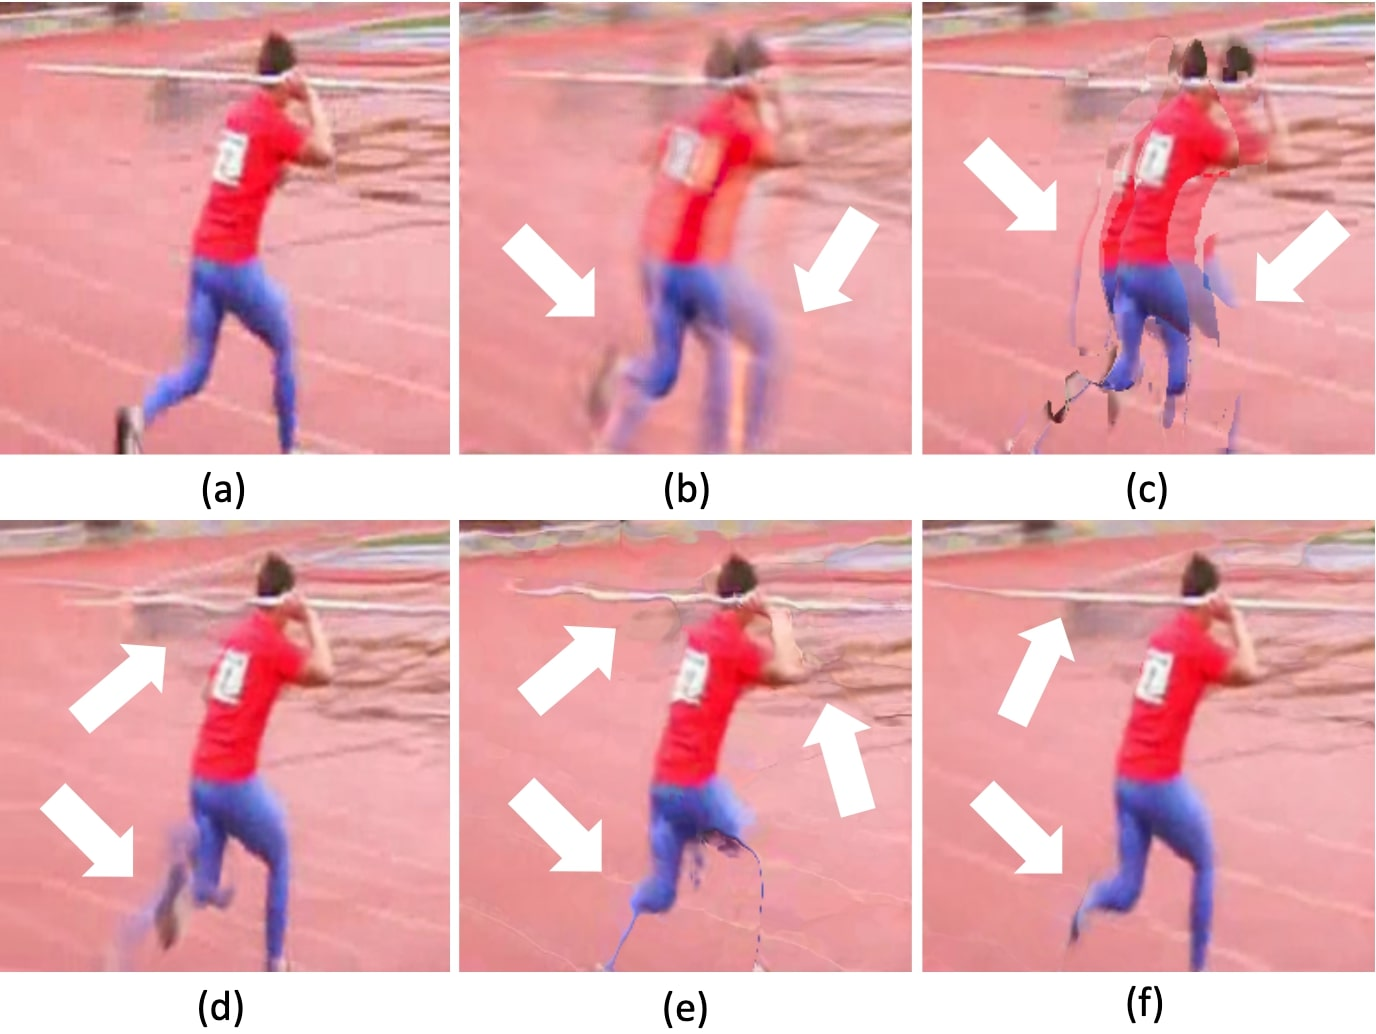
\includegraphics[width=0.7\textwidth]{img/confronto_interpolazione_frame.jpg}
    \centering
    \caption{(a) frame intermedio originale; risultati di interpolazione con: (b-e) diverse implementazioni, (f) implementazione
    di riferimento. Fonte: https://arxiv.org/abs/1712.00080}
    \label{fig:confronto_interpolazione_frame}
\end{figure}

Introduciamo brevemente il concetto delle reti neurali convoluzionali, che comunque viene toccato molto marginalmente dal
progetto (ci si limita ad utilizzare un modello prefatto).

\section*{Reti neurali convoluzionali (CNN)}

Una rete neurale può essere definita come una sequenza di \textit{layer}, ciascuno di essi formato da un'insieme di nodi (anche
detti neuroni) interconnessi tra loro. Ogni nodo è rappresentato da un peso e riceve in input un valore da ciascun nodo del layer 
precedente. Una funzione di attivazione determina lo stato di ciascun nodo: se il nodo è attivo, fornisce un input ai nodi del
layer successivo. L'output di ciascun nodo dipende dagli input e dai pesi dei nodi precedenti.

\begin{figure}[h!]
    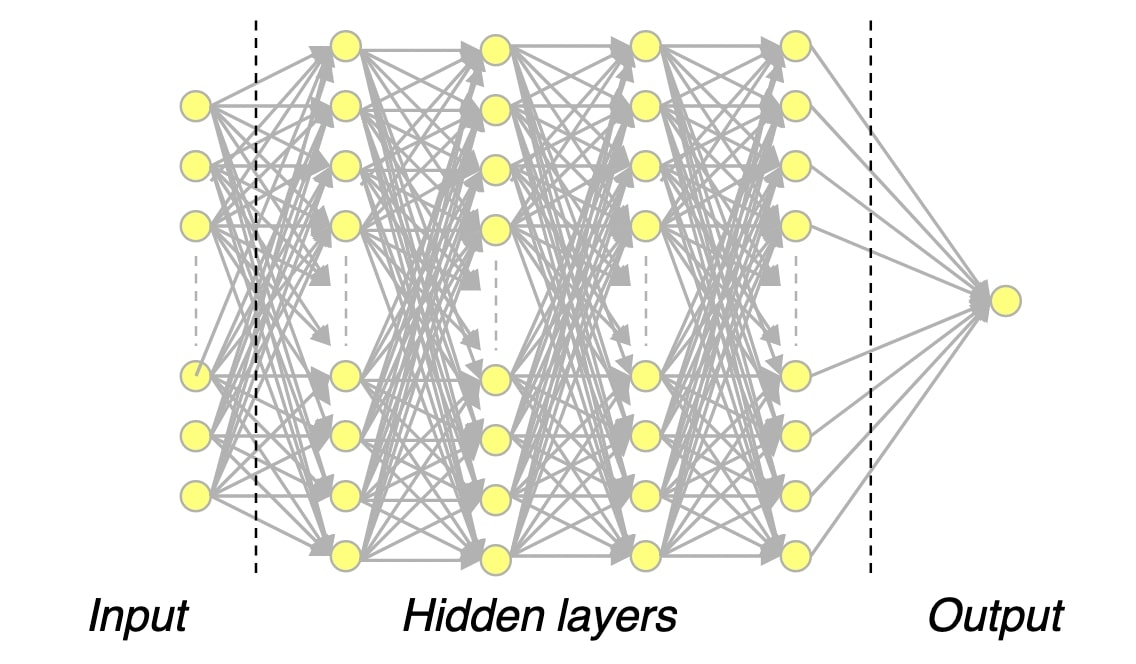
\includegraphics[width=0.5\textwidth]{img/rete_neurale.jpg}
    \centering
    \caption{Rappresentazione grafica di una rete neurale}
    \label{fig:rete_neurale}
\end{figure}

I pesi dei nodi della rete vengono assegnati secondo un processo chiamato \emph{addestramento}: vengono dati in pasto alla
rete degli input preselezionati, lasciando che i pesi iniziali (con valori casuali) forniscano l'output.
I valori dei pesi vengono poi aggiustati con l'obiettivo di minimizzare la differenza tra l'output fornito dalla rete e
l'output atteso, secondo un processo chiamato \emph{backpropagation}.

Le \textit{reti neurali convoluzionali} (CNN) sono un particolare tipo di rete neurale che trova ampio utilizzo nell'ambito
della computer vision e del processamento di immagini. Esse sono composte da tre tipi principali di layer:

\begin{itemize}
    \item Layer di Convoluzione: primo layer della rete. Può essere seguito da un layer di convoluzione o uno di pooling.
    In questi layer viene applicata la convoluzione: un filtro 2D (detto \textbf{kernel}) viene applicato all'immagine di
    input
    \item Layer di Pooling: layer intermedio (può non essere presente)
    \item Layer Fully-Connected (FC): layer finale, è l'unico in cui ciascun nodo è collegato direttamente ai nodi del
    layer precedente
\end{itemize}

Nei layer iniziali della rete viene applicata la convoluzione: un filtro 2D (\textbf{kernel}) viene passato sull'immagine
di input. L'output è di dimensioni minori dell'input e viene detto anche \textit{feature map}, poiché indica la distribuzione
di determinate caratteristiche nell'immagine. Le caratteristiche estratte sono strettamente legate al tipo di filtro utilizzato.
I layer di pooling svolgono una funzione di aggregazione dell'input, approssimando un insieme di valori adiacenti della feature
map ad un singolo valore (utilizzando un altro tipo di kernel).

La rete quindi diminuisce progressivamente le dimensioni dell'immagine di input, arrivando ad esprimere in output, ad esempio,
una probabilità. Spesso infatti, le CNN vengono utilizzate per problemi di classificazioni di immagini.
Tuttavia, come vedremo brevemente, il modello che abbiamo qui utilizzato risulta più complicato e produce un diverso tipo di 
output, non essendo adibito alla classificazione di immagini.

Nel successivo capitolo si procede a descrivere brevemente il modello Pytorch utilizzato, alcune sue caratteristiche
e il processo di conversione necessario per l'utilizzo su dispositivo Android.